\chapter{Spazi euclidei}
\section{\(E_n(\RR )\), spazio euclideo di dimensione \(n\)}
\dfn{Spazio euclideo}{Si dice \textbf{spazio euclideo} di dimensione \(n\) sul campo \(\RR \) la struttura costituita da uno spazio affine \(A_n(\RR )\) il cui spazio vettoriale \(V_n^{\circ}(\RR )\) sia dotato di un prodotto scalare "\(\cdot \)" definito positivo.}
\dfn{Ortogonalità tra sottospazi}{Siano \(S_h = [P, V_h]\) e \(S_k = [Q, V_k]\) due sottospazi lineari di \(E_{n}(\RR) \). Diremo che \(S_h\) è \textbf{ortogonale} a \(S_k\) se \[
V_h \subseteq V_k^{\perp} \quad \text{oppure} \quad V_h \supseteq V_k^{\perp}
\] }

\paragraph{Osservazione:} La relazione di ortogonalità è simmetrica. Infatti se \(S_h \perp S_k\) allora
\begin{enumerate}
    \item \(V_h \subseteq V_k^{\perp} \implies V_h^{\perp} \supseteq \left( V_k^{\perp} \right) ^{\perp} = V_k \implies V_k \subseteq V_h^{\perp} \implies S_k \perp S_h\)
    \item \(V_h \supseteq V_k^{\perp} \implies V_h^{\perp} \subseteq \left( V_k^{\perp} \right) ^{\perp} = V_k \implies V_k \supseteq V_h^{\perp} \implies S_h \perp S_k\)
\end{enumerate}
In entrambi i casi \(S_h \perp S_k \iff S_k \perp S_h\). Quindi diremo semplicemente che \(S_h\) e \(S_k\) sono ortogonali.

\mprop{}{In \(E_2(\RR )\), dati la retta \(r\) e il punto \(H\), esiste un'unica retta passante per \(H\) e ortogonale a \(r\).}
\pf{Dimostrazione}{Dimostriamo prima di tutto l'esistenza della retta, successivamente ci occuperemo dell'unicità. Poniamo \(r : [P, V_1]\) e definiamo una \(s : [H, V_1^{\perp}]\). \(s\) è una retta poiché \(\RR ^{2} = V_1 \oplus V_1^{\perp}\), per la formula di Grassmann \(V_1^{\perp}\) ha dimensione 1, quindi \(s\) è una retta. \(H \in s\) per costruzione e \(r \perp s\) perché \(V_1^{\perp} \subseteq V_1^{\perp}\), cioè lo spazio di traslazione della retta \(s\) contiene la direzione ortogonale a \(V_1\). Ora l'unicità della retta segue dall'unicità dello spazio di traslazione e poiché esso ha dimensione 1, anche la retta è unica.}

\mprop{}{In \(E_3(\RR )\), siano assegnati una retta \(r\) e un piano \(\alpha \). Dato un punto \(H\) 
\begin{enumerate}
    \item esiste un'unica retta \(s\) passante per \(H\) e ortogonale al piano \(\alpha \)
    \item esiste un unico piano \(\beta \) passante per \(H\) e ortogonale alla retta \(r\)
\end{enumerate}}
\newpage
\pf{Dimostrazione}{Dimostriamo i 2 punti separatamente
\begin{enumerate}
    \item poniamo \(\alpha = [P, V_2]\) e \(s = [H, V_2^{\perp}]\). \(s\) è una retta perché \(\dim(V_2^{\perp}) = 1\), poiché \(\RR^{3} = V_2 \oplus V_2^{\perp}\) per la formula di Grassmann. \(H \in s\) e \(s \perp\alpha \) valgono per costruzione.
    \item poniamo \(r = [Q, V_1]\) e definiamo \(\beta = [H, V_1^{\perp}]\). Verifichiamo che \(\beta \) sia un piano. Osserviamo che dato che  \[
    \underbrace{\RR ^{3}}_{3} = \underbrace{V_1}_{1} \oplus \underbrace{V_1^{\perp}}_{2}  \implies \dim(V_1^{\perp}) = 2
    \] quindi \(\beta \) è un piano. \(H \in \beta \) e \(\beta \perp r\) valgono per costruzione. L'unicità del piano segue dall'unicità di \(V_2\) di dimensione 2 e perpendicolare a \(V_1\).
\end{enumerate}}

\mprop{}{Siano \(r: [P, V_1]\) e \(\alpha = [Q, V_2]\) rispettivamente una retta e un piano di \(E_3(\RR )\). Se \(r \perp \alpha \) abbiamo che
\begin{enumerate}
    \item \(r \perp s \quad \forall s \subseteq \alpha \), cioè \(r\) è perpendicolare a ogni retta \(s\) contenuta nel piano \(\alpha \)
    \item \(\alpha \perp \beta \quad \forall \beta \supseteq r\), cioè \(\alpha \) è perpendicolare a ogni piano \(\beta \) contenente \(r\)
\end{enumerate}}

\pf{Dimostrazione}{Dimostriamo i 2 punti separatamente
\begin{enumerate}
    \item Sia \(s \subseteq \alpha \) con \(s = [H, V_1']\), allora  \[
    \underbrace{V_1' \subseteq V_2}_{\text{poiché } s \subseteq \alpha } = \underbrace{V_1^{\perp}}_{\text{poiché } r \perp s} \implies r \perp s
    \] 
    \item Sia \(\beta \subseteq \alpha \) con \(\beta = [H, V_2']\), allora  \[
    \underbrace{V_2' \supseteq V_1}_{\text{poiché } \beta \supseteq r } = \underbrace{V_2^{\perp}}_{\text{poiché } r \perp \alpha } \implies \alpha \perp \beta
    \] 
\end{enumerate}}

\mprop{}{Siano \(\alpha\) e \(r\) rispettivamente un piano e una retta di \(E_3(\RR)\), con \(\alpha \) non ortogonale a \(r\). Allora esiste un unico piano \(\beta\) ortogonale ad \(\alpha\) e contenente la retta \(r\).}

\pf{Dimostrazione}{Sia \(\beta = [P, V_1 \oplus V_2^{\perp}]\) dove \(r = [P, V_1]\) e \(\alpha = [Q, V_2]\). \(\beta\) è un piano perché \(\dim(V_1) = 1, \ \dim(V_2^{\perp})= 1\) e \(V_1 \neq V_2^{\perp}\) (poiché \(\alpha \not\perp r\) ) \( \implies \dim(V_1 \oplus V_2^{\perp}) = 2 \implies \beta\) è un piano. Per costruzione abbiamo che \(\beta \perp \alpha\), infatti lo spazio di traslazione di \(\beta\) è: \[
        V_1 \oplus V_2^{\perp} \supseteq V_2^{\perp} \text{  }
    \] e \(V_2\) è lo spazio di traslazione di \(\alpha\). Inoltre \(\beta \) contiene \(r\) per le proposizioni precedenti ed è ovviamente ortogonale a \(\alpha \). Per costruzione \(\beta \) è l'unico piano che soddisfa queste condizioni.}

\section{Geometria analitica in \(E_n(\RR)\) }
\dfn{}{In \(E_n(\RR)\) si dice \textbf{riferimento cartesiano ortogonale monometrico} la coppia \(RC = [O, \mcB]\) dove \(O\) è un punto di \(E_n(\RR)\) e \(\mcB=(e_1, e_2, ..., e_n)\) è una base ortonormale.}
\newpage
\nt{\begin{enumerate}
    \item In \(E_2(\RR)\) si conviene indicare la base ortonormale come \(\mcB = (i,j)\) 
    \item In \(E_3(\RR)\) si conviene indicare la base ortonormale come \(\mcB = (i,j, k)\) 
\end{enumerate}}

\section{Ortogonalità}
\subsubsection{Ortogonalità fra rette}
Siano \(r_1, r_2\) due rette di \(E_2(\RR)\) e sia \(r_1 = [P, f(v)]\) con \(v = li + mj\), analogamente \(r_2 = [P, f(v')]\) con \( v' = l'i + m'j\) \[
    v \perp v' \iff ll' + mm' = 0
    \] se \(r_1\) ha equazione \(ax + by + c = 0\) e \(r_2\) ha equazione \(a'x + b'y + c' = 0\) allora \(P.d.r_1 = [(-b,a)]\), e \(P.d.r_2 = [(-b', a')]\) quindi \[
    r_1 \perp r_2 \iff -b (-b') + aa' = bb' + aa' = 0
\]
Se abbiamo due rette \(r_1, r_2\) in \(E_3(\RR)\) con \(p.d.r_1 = [(l,m,n)]\), \(p.d.r_2 = [(l',m',n')]\) allora \(r_1 \perp r_2 \iff v_1\), cioè il generatore della direzione della retta \(r_1\), è ortogonale a \(v_2\), che è generatore della direzione della retta \(r_2\). \[
    v_1 = li + mj + nk \qquad v_2 = l'i + m'j + n'k
\] \[
    v_1 \perp v_2 \iff r_1 \perp r_2 \iff ll' + mm' + nn' = 0
\] Analogamente se \(r_1, r_2\) sono rette in \(E_n(\RR)\) con \(p.d.r_1 = [(x_1, x_2, ..., x_n)]\), \(p.d.r_2 = [(x_1', x_2', ..., x_n')]\) \[
r_1 \perp r_2 \iff x_1x_1' + x_2 x_2' + \ldots  + x_n x_n' = 0
\] 

\subsubsection{Direzione ortogonale a un iperpiano}
\mprop{}{Sia \(r: ax + by + c = 0\) una retta di \(E_2(\RR)\), allora \([(a, b)]\) è la classe dei parametri direttori della direzione ortogonale a \(r\).}
\pf{Dimostrazione}{Per ipotesi \(p.d.r = [(-b,a)]\) e abbiamo che per essere ortogonale la direzione \((a, b)(-b, a)= 0\) oppure equivalentemente \((ai + bj)( -b i + aj ) = 0 \implies [(a, b)] \perp r\).  }
\mprop{}{Sia \(\pi: ax + by + cz + d = 0\) un piano in \(E_3(\RR)\), allora \([(a, b, c)]\) è la classe dei parametri direttori della direzione ortogonale a \(\pi\).}
\pf{Dimostrazione}{Sia \(v \in V_2\) tale che \(\pi\) ha spazio di traslazione \(V_2\). Se \(v = (x, y, z) \implies ax + by + cz = 0 \iff (x, y, z)(a, b, c) = 0 \implies (a,b,c) \perp v \ \forall v \in V_2 \) }
\mprop{}{Più in generale: sia \(S _{n-1}\) un iperpiano in \(E_n(\RR)\) di equazione cartesiana \(a_1 x_1 + a_2 x_2 + ... + a_n x_n + a_0 = 0 \implies [(a_1, a_2, ..., a_n)]\) è la classe dei parametri direttori della direzione ortogonale a \(S _{n-1}\).}

\subsubsection{Ortogonalità fra piani in \(E_3(\RR )\)}
\mprop{}{Siano \(\alpha: ax + by + cz + d = 0\) e \(\beta: a'x + b'y + c'z + d' = 0\) due piani in \(E_3(\RR)\), con \((a,b,c) \neq (0,0,0)\), allora \(\alpha \perp \beta \iff a a' + b b' + c c' = 0\) }
\pf{Dimostrazione}{\(\alpha \perp \beta \iff V_2 \supseteq V_2'^{\perp}\) dove \(V_2\) è la giacitura di \(\alpha\) e \(V_2'\) è la giacitura di \(\beta\). \[V_2'^{\perp}= [\mcL((a', b',c')) ] \iff (a', b', c') \in V_2\]
\((x, y, z) \in V_2 \iff ax + by + cz = 0\) e quindi \((a', b', c') \in V_2 \iff a a' + b b' + c c' = 0\) }
\subsubsection{Ortogonalità fra retta e piano in \(E_3(\RR )\)}
\mprop{}{In \(E_3(\RR)\), sia \(r\) una retta con \(p.d.r = [(l,m,n)]\) e sia \(\alpha\) un piano di equazione \(ax + by + cz + d= 0\), allora \(r \perp \alpha\) se, e soltanto se, \([(a,b,c)] = [(l,m,n)]\) }
\pf{Dimostrazione}{\(r \perp \alpha \iff V_1=V_2^{\perp}\) dove \(V_1\) è la direzione della retta e \(V_2\) è la giacitura di \(\alpha\). \[
        V_1 = \mcL((l,m,n)) = V_2 ^{\perp} = \mcL((a,b,c)) \iff [(a,b,c)] = [(l,m,n)]  
\]}

\section{Distanza}
\subsubsection{Distanza fra due punti in \(E_n(\RR )\)}
Siano \(P = (x_{1} , x_{2}, ..., x_{n} )\) e \(Q = (x_{1} ' x_2 ', ..., x_n ')\). La distanza tra \(P\) e \(Q\) è la norma del vettore \(\vec{PQ}\), quindi\[
        d(P,Q) = ||\vec{PQ}|| = \sqrt{\vec{PQ} \cdot \vec{PQ}}
\]     \[
    \vec{{PQ}} = (x_1'-x_1) e_1 + ... + (x_n' - x_n) e_n
\] \[
    d(P,Q) = ||\vec{{PQ}}|| = \sqrt{(x_1' - x_1)^{2} + ... + (x_n'-x_n)^{2}  }
\]
\begin{enumerate}
    \item In \(E_{2}(\RR)\), dati \(P = (x, y) \) e \( Q = (x', y')\)\[
    \vec{{PQ}} = (x'- x) i + (y' - y)j
\] \[
    d (P, Q) = \sqrt{(x' - x)^{2} + (y'-y)^{2} }
\] 
    \item In \(E_{3}(\RR)\), dati \(P = (x, y,z) \) e \( Q = (x', y',z')\)\[
    \vec{{PQ}} = (x'- x) i + (y' - y)j + (z' - z)k
\] \[
    d (P, Q) = \sqrt{(x' - x)^{2} + (y'-y)^{2}  + (z' - z ) ^2}
\] 
\end{enumerate}
\subsubsection{Distanza punto retta in \(E_2(\RR )\)}
Siano \(P = (x_0, y_0)\) e \(r = [Q, V_1]\) rispettivamente un punto e una retta in \(E_{2}(\RR)\). Definiamo la distanza tra il punto \(P\) e la retta \(r\) come la distanza tra \(P\) e il punto \(H\), piede della perpendicolare per \(P\) a \(r\) (cioè l'intersezione tra \(r\) e la retta perpendicolare a \(r\) passante per \(P\)). 
\begin{center}
    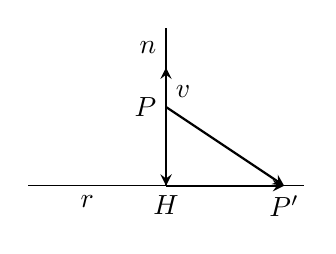
\begin{tikzpicture}[scale = 0.5]
        \coordinate (P) at (0, 0);
        \coordinate (H) at (0, -2);
        \coordinate (P') at (3, -2);
        \draw[thick, -stealth] (P) -- (H); 
        \draw[thick, -stealth] (P) -- (0, 1); 
        \draw[thick, -stealth] (P) -- (P'); 
        \draw[thick, -stealth] (H) -- (P'); 
        \draw[thin] (-3.5, -2) -- (3.5, -2);
        \draw[thin] (0, 2) -- (0, -2);
        \node[below] at (P') {\(P'\)};
        \node[below] at (H) {\(H\)};
        \node[below] at (-2, -2) {\(r\)};
        \node[left] at (P) {\(P\)};
        \node[left] at (0, 1.5) {\(n\)};
        \node[right] at (0, 0.4) {\(v\)};
    \end{tikzpicture}
\end{center}
Determiniamo \(||\vec{{PH}}||\). Se \(r\) ha equazione \(ax + by +c = 0\) allora \(V_1^{\perp} = \mcL(a i + b j)  \). Posta \[n = [P, V_1^{\perp}] \implies n = [P, \mcL(a i + bj) ]\]
\(H = n \cap r \) è la proiezione di \(P\) su \(r\) (cioè l'intersezione tra \(r\) e la retta per \(P^{\perp} \)). Sia \(P' = (x', y')\) un generico punto su \(r\) di equazione \(ax + by + c = 0\). \(PH\) è la componente di \(PP'\) lungo \(v\). \[PP' = (x'-x_0) i + (y' - y_0)j\]\[
    \vec{{PH}} = \frac{\vec{PP'} \cdot v}{ v \cdot v } v
\] \[
d(P,r) = d (P, H) = || \vec{{PH}} || = \left\| \left( \frac{\vec{{PP'}} \cdot v}{v \cdot v} v \right)  \right\| = \frac{|\vec{PP'} \cdot v| }{\|v\|} = \frac{|(x'-x_0) a + (y' - y_0) b| }{\sqrt{a^2 + b ^2} } = \frac{|x'a + y'b - x_0a - y_0b| }{\sqrt{a^2 + b ^2} }
\] e, dato che \(P'\) appartiene a \(r\) e che, quindi, \(ax' + by' = -c\), si ha \[
d(P, r) = \frac{|ax_0 + by_0 + c|}{\sqrt{a^{2} + b^{2} }}
\] 
\subsubsection{Distanza punto piano in \(E_3(\RR )\)}
Siano \(P = (x_0, y_0, x_0)\) e \(\alpha : ax + by + cz + d = 0\) rispettivamente un punto e un piano di \(E_{3}(\RR)\). Definiamo la distanza \(d(P, \alpha)\) come la distanza tra \(P\) e il punto \(H\), intersezione tra \(\alpha\) e la retta per \(p \perp \alpha \). Infatti \(d(P, \alpha )= d (P, H) = ||\vec{{PH}}||\). Analogamente al caso precedente abbiamo che \[
    d(P, \alpha ) = \frac{|ax_0 + by_0 + cz_0 + d|}{\sqrt{a^{2} + b^{2} + c^{2} }}
\]

\subsubsection{Distanza punto retta in \(E_{3}(\RR)\) }
Siano \(P\) e \(r = [Q, V_1]\) rispettivamente un punto e una retta in \(E_{3}(\RR)\). Sia \(\alpha \) il piano per \(P\) ortogonale a \(r\) e sia \(H\) l'intersezione tra \(r\) e \(\alpha \). Definiamo \(d(P, r) = d(P, H) = ||\vec{{PH}}||\).

\ex{}{In \(E_{3}(\RR)\) determiniamo la distanza di \(P = (3, 0, 1)\) da \(r : 
\begin{cases}
    x + y = 1 \\
    z = 2 \\
\end{cases}
\)  \[
\begin{cases}
    x = 1-t \\
    y = t \\
    z = 2 \\
\end{cases} \quad P.d.r = [(-1, 1, 0)]=[(a,b,c)] \qquad \alpha: -x + y + 0 \cdot z + d = 0
\] \[
    \text{ Imponiamo il passaggio per \(P\)}: \quad -3 + 0 + d = 0 \quad d = 3 \quad \alpha : -x + y + 3 = 0
\] \[
    \alpha \cap r :
\begin{cases}
    x + y = 1 \\
    -x + y + 3 = 0 \\
    z = 2 \\
\end{cases} \quad
\begin{cases}
    x+y=1 \\
    0x + 2y= -2 \\
    z=2 \\
\end{cases} \implies x = 2; \ y = -1
\]\[
    H: (2, -1, 2) \quad d(P,r) = ||\vec{{PH}}|| = \vec{{PH}} = (-1) i + (-1) j + k = -1 -j + k
\]}

\subsubsection{Distanza tra due rette sghembe in \(E_3(\RR )\)}
\dfn{Retta di minima distanza}{Si dice \textbf{retta di minima distanza} tra due rette \(r\) e \(s\) sghembe in \(E_{3}(\RR)\) una retta ortogonale e incidente sia ad \(r\) che ad \(s\).}

\dfn{Distanza tra due rette sghembe in \(E_{3}(\RR)\)}{Definiamo \textbf{la distanza tra due rette \(r\) e \(s\) sghembe} in \(E_{3}(\RR)\) come la distanza tra i punti \(R\) e \(S\) ottenuti intersecando la retta \(t\) di minima distanza tra \(r\) e \(s\) con \(r\) e \(s\).}

\mprop{}{La retta di minima distanza tra \(r\) e \(s\) esiste ed è unica.}

\subsubsection{Assi e piani assiali}
\dfn{Asse}{In \(E_{2}(\RR)\) dati due punti \(P,Q\), si dice \textbf{asse} del segmento \([P,Q]\) la retta passante per il punto medio di \(P\) e \(Q\) e ortogonale alla retta per \(P\) e \(Q\).}
\mprop{}{L'asse di un segmento \([P,Q]\) è il luogo dei punti equidistanti da \(P\) e da \(Q\).}
\pf{Dimostrazione}{Dobbiamo dimostrare che \(||\vec{PH} || = ||\vec{QH} || \quad \forall H \in a\) (asse di \([P,Q]\)). \[
    \vec{PH} = \vec{PM} + \vec{MH} \quad e \quad \vec{QH} = \vec{QM} + \vec{MH} 
\] \[
    ||\vec{PH} || = \sqrt{||PM || ^{2} + ||MH||^{2}  } \quad ||\vec{QH} || = \sqrt{||QM|| ^{2} + ||MH|| ^{2} } \quad \text{ ma } \quad ||PM||= ||QM|| 
\] \[
    ||\vec{PH} || = \sqrt{||PM|| ^{2} + ||MH|| ^{2} } = \sqrt{||QM|| ^{2} + ||MH|| ^{2} } = ||\vec{QH} || 
\]}

\ex{}{Determiniamo l'asse di \(P=(1,1)\) e \(Q=(2, -4)\). Il punto \(M = (\frac{3}{2}, -\frac{3}{2})\) \[
    \vec{PQ} = (2-1) i + (-4-1) j = 1 - 5 j = (1, -5)
\] \(r \perp \vec{PQ} \) per \(M\)  è del tipo \[
    x -5y + c = 0 \quad \text{e passa per \(M\) }
\] \[
    \frac{3}{2} + \frac{15}{2} + c = 0 \quad c = -9 \implies r : \ x - 5y -9 = 0
\]Alternativamente \[
    r: \ H \in r \iff d(H,P) = d(H, Q)
\]se \(H = (x, y)\) \[
    \sqrt{(x-1)^{2} + (y-1) ^{2} } = \sqrt{(x-2)^{2} + (y + 4)^{2} }
\] \[
    x^{2} - 2x + 1 + y^{2}  -2y + 1 = x^{2} - 4x + 4 + y^{2} + 8y + 16 \implies r: \ 2x -10y -18 = 0
\]}

\dfn{Piano assiale}{In \(E_{3}(\RR)\) si dice \textbf{piano assiale} del segmento \([P,Q]\) il piano \(\alpha \) passante per il punto medio di \(P\) e \(Q\) e ortogonale al segmento \([P,Q]\).}

\mprop{}{Il piano assiale del segmento \([P,Q]\) è il luogo dei punti equidistanti tra \(P\) e \(Q\).}

\section{Circonferenza e sfera}
\dfn{Circonferenza}{Dato un punto \(C = (x_0, y_0)\) in \(E_{2}(\RR)\) e dato \(r\), numero reale positivo, si dice \textbf{circonferenza} di centro \(C\) e raggio \(r\) il luogo dei punti aventi distanza \(r\) da \(C\). }
\dfn{Sfera}{Sia \(C = (x_{0}, y_{0}, z_{0} )\) e sia \(r\) un numero reale positivo. Si dice \textbf{sfera} di raggio \(C\) e di centro \(r\) il luogo dei punti aventi distanza \(r\) da \(C\).}
\paragraph{Osservazione:} La circonferenza è una curva algebrica reale, mentre la sfera è una superficie algebrica reale.
\subsubsection{Rappresentazione analitica di una circonferenza in \(E_2(\RR )\)}
Sia il generico punto \(P=(x, y)\) appartenente alla circonferenza di centro \(C = (x_0, y_0)\) e raggio \(r\). \[
d(P,C) = \sqrt{(x-x_0)^{2} + (y-y_0)^2} = \sqrt{x^{2} + y^{2} + 2ax + 2by + x_0^2 + y_0^2} = r \iff (x-x_0)^{2} + (y-y_0)^{2} = r^{2}  
\] \[
    x^{2} + y^{2} + 2ax + 2by + c = 0 \iff x^{2} + y^{2} - 2x_0x - 2y_0y + (x_0^{2} + y_0^{2} - r^{2} ) = 0
\] 

\mprop{Equazione cartesiana di una circonferenza}{Tutte e sole le circonferenze si rappresentano come \[x^{2} + y^{2} + 2ax + 2by + c = 0 \quad \text{con} \quad a^{2} + b^{2} - c > 0\] e avremo che \(C = (-a, -b)\) e \(r = \sqrt{a^{2} + b^{2} -c}\)  }

\nt{Se \(r\) fosse 0 allora \(a^{2} + b^{2} - c = 0\) e quindi \(x^{2} + y^{2} + 2ax + 2by + c = 0\) rappresenta il solo punto \(C = (-a, -b)\).}
\mprop{}{Per tre punti non allineati in \(E_{2}(\RR)\) passa un'unica circonferenza.}

\subsubsection{Rappresentazione analitica di una sfera in \(E_3(\RR )\)}
Sia il generico punto \(P = (x,y,z)\) appartenente alla sfera, allora \[
    d(P,C) = \sqrt{(x-x_0)^{2} + (y-y_0)^{2} + (z-z_0)^{2}} = r \iff (x-x_0)^{2} + (y-y_0)^{2} + (z-z_0)^{2} = r^{2}
\]
\mprop{Equazione cartesiana di una sfera}{Tutte e sole le sfere si rappresentano come \[x^{2} + y^{2} + z^{2} + 2ax + 2by + 2cz + d = 0 \quad \text{con} \quad a^{2} + b^{2} + c^{2} > 0\] e avremo che \(C = (-a, -b, -c)\) e \( r = \sqrt{a^{2} + b^{2} + c^{2} - d}\)  }
\nt{Se \(a^{2} + b^{2} + c^{2} - d = 0\) allora \(x^{2} + y^{2} + z^{2} + 2ax + 2by + 2cz + d = 0\) è realizzata dal solo punto \(C = (-a, -b, -c)\). }

\mprop{}{Per quattro punti non complanari di \(E_{3}(\RR)\) passa un'unica sfera.}

\subsubsection{Circonferenze in \(E_{3}(\RR)\) }
\dfn{Circonferenza in \(E_{3}(\RR)\) }{In \(E_3(\RR )\) dati un piano \(\alpha \), un suo punto \(C\) e un numero reale positivo \(r\), si dice \textbf{circonferenza} di centro \(C\) e raggio \(r\) il luogo dei punti di \(\alpha \) aventi distanza \(r\) da \(C\).}

\paragraph{Osservazione:} Una circonferenza appartiene a infinite sfere. Quindi per tre punti non allineati passano infinite sfere.

\mprop{}{Tutte e sole le circonferenze di \(E_{3}(\RR)\) ammettono una rappresentazione del tipo \[
\begin{cases}
    \ ax + by + cz + d = 0 \quad \rightarrow \quad \text{piano \(\alpha \) } \\
    \ (x- x_0)^{2} + (y - y_0)^{2} + (z-z_0)^{2} = R^{2} \\ 
\end{cases}
\] \[
    d(C', \alpha ) < R \quad \text{ove} \quad C' = (x_0, y_0, z_0) \quad e \quad 
    \frac{|ax_0 + by_0 + cz_0 + d| }{\sqrt{a^{2} + b^{2} + c^{2} }} < R
\]}
\paragraph{Osservazione:} Vi sono infinite sfere che intersecano la circonferenza, ma solo in una di esse il centro \(C'\) della sfera coincide con il centro \(C\) della circonferenza.
Il centro della circonferenza \(C\) si trova intersecando il piano \(\alpha \) con la retta per il centro della sfera \(C'\) perpendicolarmente ad \(\alpha \). Per determinare il raggio della circonferenza utilizziamo il teorema di Pitagora. Conosciamo sia \([C,C'] = h\) che il raggio \(R\) della sfera. Quindi \[
    r = \sqrt{R^{2} - h^{2}}
\]
\begin{figure}[ht]
    \centering
    \def\svgwidth{130pt}
    \incfig{circonferenza-tridimensionale}
    \label{fig:circonferenza-tridimensionale}
\end{figure}
\nt{Una circonferenza in \(E_3(\RR )\) si può ottenere anche intersecando anche altre superfici con un piano, non solo una sfera.}

\ex{}{Determinare se la seguente è una circonferenza \[
\begin{cases}
    x^{2} + y^{2} = 7 \\
    z = 3 \ \rightarrow \ \alpha \\
\end{cases}
\] \[
    x^{2} + y^{2} + z^{2} - z^{2} = 7 \quad  \text{ e siccome \(z = 3\)} \quad 
\begin{cases}
    x^{2} + y^{2} + z^{2} = 16 \\
    z = 3 \\
\end{cases} \text{ che descrive una circonferenza.}
\]}
